\section{Comment bootstrapper}

\subsection{Un exemple concret : le langage OCaml}
\begin{frame}
    \frametitle{Un exemple concret : le langage OCaml\esp}

    \hbox{
        \begin{minipage}{.3\textwidth}
            \centering
            \boxed{\texttt{ocamlc}}
        \end{minipage}
        \begin{minipage}{.3\textwidth}
            \centering
            Librairie standard
        \end{minipage}
        \begin{minipage}{.3\textwidth}
            \centering
            \boxed{\texttt{ocamlrun}}
        \end{minipage}
    }

    \vspace{0.5cm}

    \uncover<2->{
        Code source OCaml: \url{https://github.com/ocaml/ocaml.git}
    }

    \vspace{.2cm}

    \uncover<3->{
        \boxed{
            \hbox{
                \begin{minipage}{.3\textwidth}
                    \centering
                    Code source \texttt{ocamlc} en \textbf{OCaml}
                \end{minipage}
                \begin{minipage}{.3\textwidth}
                    \centering
                    Code source de la librairie standard en \textbf{C} et en \textbf{OCaml}
                \end{minipage}
                \begin{minipage}{.3\textwidth}
                    \centering
                    Code source \texttt{ocamlrun} en \textbf{C}
                \end{minipage}
            }
        }
    }

    \vspace{0.5cm}

    \uncover<4->{
        \begin{center}
            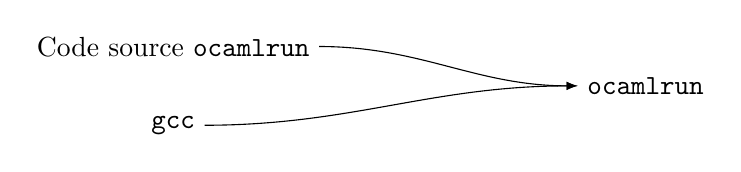
\begin{tikzpicture}[in=180,out=0]
                \node (ocamlrun_source) at (-3, 0.5) {Code source \texttt{ocamlrun}};
                \node (gcc) at (-3, -0.5) {\boxed{\texttt{gcc}}};
                \node (ocamlrun) at (3, 0) {\boxed{\texttt{ocamlrun}}};

                \draw[-latex] (gcc.east) to (ocamlrun.west);
                \draw[-latex] (ocamlrun_source.east) to (ocamlrun.west);
            \end{tikzpicture}
        \end{center}
    }

    \uncover<5->{
        \begin{center}
            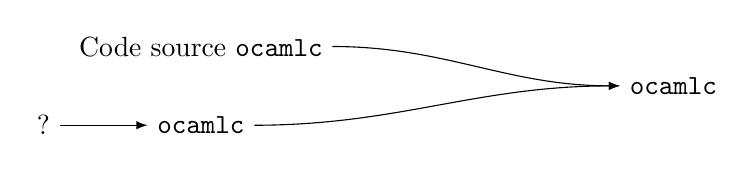
\begin{tikzpicture}[in=180,out=0]
                \node (ocamlc_source) at (-3, 0.5) {Code source \texttt{ocamlc}};
                \node (ocamlc_pre) at (-3, -0.5) {\boxed{\texttt{ocamlc}}};
                \node (ocamlc_post) at (3, 0) {\boxed{\texttt{ocamlc}}};
                \node (how) at (-5, -0.5) {?};

                \draw[-latex] (ocamlc_pre.east) to (ocamlc_post.west);
                \draw[-latex] (ocamlc_source.east) to (ocamlc_post.west);
                \draw[-latex] (how.east) to (ocamlc_pre.west);
            \end{tikzpicture}
        \end{center}
    }
\end{frame}

\subsection{Premiere méthode : les cycles de bootstrapping}
\begin{frame}
    \frametitle{Premiere méthode : les cycles de bootstrapping\esp}

    \begin{center}
        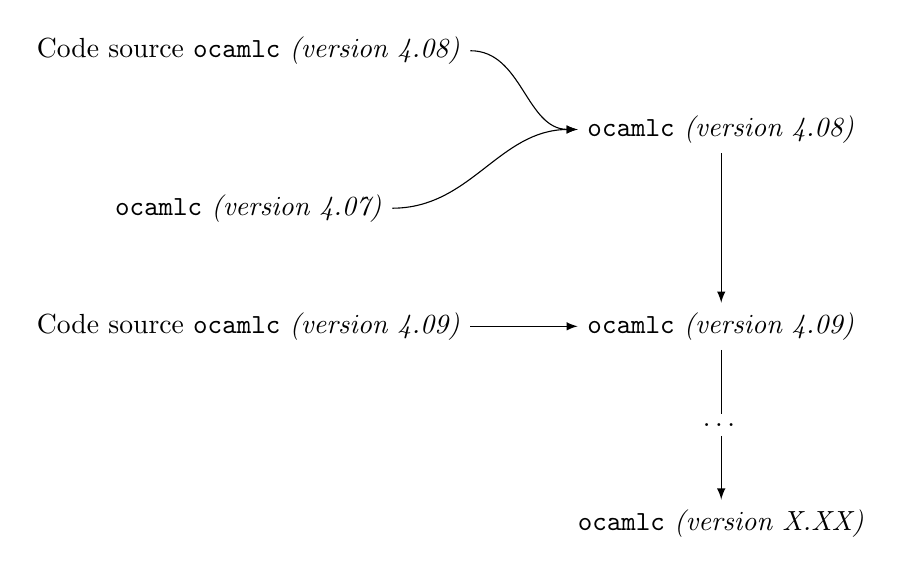
\begin{tikzpicture}[in=180,out=0]
            \node (ocamlc_source_407) at (-3, 1) {Code source \texttt{ocamlc} \emph{(version 4.08)}};
            \node (ocamlc_407) at (-3, -1) {\boxed{\texttt{ocamlc}} \emph{(version 4.07)}};

            \uncover<2->{
                \node (ocamlc_408) at (3, 0) {\boxed{\texttt{ocamlc}} \emph{(version 4.08)}};

                \draw[-latex] (ocamlc_407.east) to (ocamlc_408.west);
                \draw[-latex] (ocamlc_source_407.east) to (ocamlc_408.west);
            }

            \uncover<3->{
                \node (ocamlc_source_409) at (-3, -2.5) {Code source \texttt{ocamlc} \emph{(version 4.09)}};
            }

            \uncover<4->{
                \node (ocamlc_409) at (3, -2.5) {\boxed{\texttt{ocamlc}} \emph{(version 4.09)}};

                \draw[-latex] (ocamlc_source_409.east) to (ocamlc_409.west);
                \draw[-latex] (ocamlc_408.south) to [out=-90,in=90] (ocamlc_409.north);
            }

            \uncover<5->{
                \node (ocamlc_any) at (3, -5) {\boxed{\texttt{ocamlc}} \emph{(version X.XX)}};
                \node (iterations) at (3, -3.75) {\dots};

                \draw (ocamlc_409.south) to [out=-90,in=90] (iterations.north);
                \draw[-latex] (iterations.south) to [out=-90,in=90] (ocamlc_any.north);
            }
        \end{tikzpicture}
    \end{center}
\end{frame}

\subsection{Deuxième méthode : le bootstrapping "direct"}
\begin{frame}
    \frametitle{Deuxième méthode : le bootstrapping "direct"\esp}
    \begin{center}
        \only<1>{
            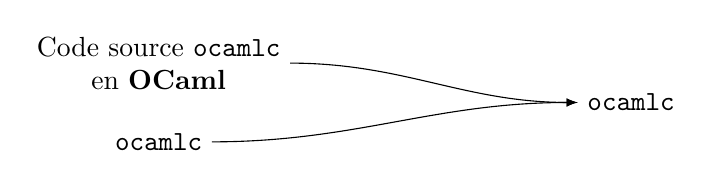
\begin{tikzpicture}[in=180,out=0]
                \node [align=center] (ocamlc_source) at (-3, 0.5) {
                    Code source \texttt{ocamlc} \\
                    en \textbf{OCaml}
                };
                \node (ocamlc_pre) at (-3, -0.5) {\boxed{\texttt{ocamlc}}};
                \node (ocamlc_post) at (3, 0) {\boxed{\texttt{ocamlc}}};

                \draw[-latex] (ocamlc_pre.east) to (ocamlc_post.west);
                \draw[-latex] (ocamlc_source.east) to (ocamlc_post.west);
            \end{tikzpicture}
        }
        \only<2->{
            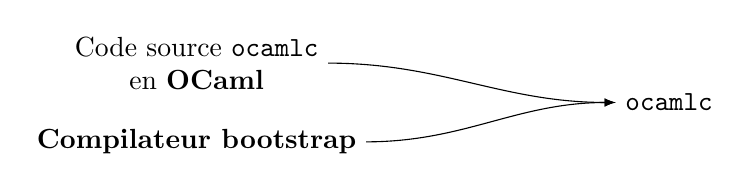
\begin{tikzpicture}[in=180,out=0]
                \node [align=center] (ocamlc_source) at (-3, 0.5) {
                    Code source \texttt{ocamlc} \\
                    en \textbf{OCaml}
                };
                \node (ocamlc_post) at (3, 0) {\boxed{\texttt{ocamlc}}};

                \draw[-latex] (ocamlc_source.east) to (ocamlc_post.west);

                \uncover<3->{
                    \node (bootstrap_compiler) at (-3, -0.5) {\textbf{Compilateur bootstrap}};

                    \draw[-latex] (bootstrap_compiler.east) to (ocamlc_post.west);
                }
            \end{tikzpicture}

            \vspace{1cm}

            \uncover<4->{
                \begin{itemize}
                    \item Ancienne version du compilateur (ici, \texttt{ocamlc})
                          écrite en un autre langage.
                    \item Compilateur/interpr\'eteur simpliste voué
                          explicitement au bootstrapping du compilateur.
                \end{itemize}
            }
        }
    \end{center}
\end{frame}
